\documentclass[10pt, a5paper]{article}
\usepackage{pdfpages}
\usepackage{parallel}
\usepackage[T2A]{fontenc}
\usepackage{ucs}
\usepackage[utf8x]{inputenc}
\usepackage[polish,english,russian]{babel}
\usepackage{hyperref}
\usepackage{rotating}
\usepackage[inner=2cm,top=1.8cm,outer=2cm,bottom=2.3cm,nohead]{geometry}
\usepackage{listings}
\usepackage{graphicx}
\usepackage{wrapfig}
\usepackage{longtable}
\usepackage{indentfirst}
\usepackage{array}
\newcolumntype{P}[1]{>{\raggedright\arraybackslash}p{#1}}
\frenchspacing
\usepackage{fixltx2e} %text sub- and superscripts
\usepackage{icomma} % коскі ў матэматычным рэжыме
\PreloadUnicodePage{4}

\newcommand{\longpage}{\enlargethispage{\baselineskip}}
\newcommand{\shortpage}{\enlargethispage{-\baselineskip}}

\def\switchlang#1{\expandafter\csname switchlang#1\endcsname}
\def\switchlangbe{
\let\saverefname=\refname%
\def\refname{Літаратура}%
\def\figurename{Іл.}%
}
\def\switchlangen{
\let\saverefname=\refname%
\def\refname{References}%
\def\figurename{Fig.}%
}
\def\switchlangru{
\let\saverefname=\refname%
\let\savefigurename=\figurename%
\def\refname{Литература}%
\def\figurename{Рис.}%
}

\hyphenation{admi-ni-stra-tive}
\hyphenation{ex-pe-ri-ence}
\hyphenation{fle-xi-bi-li-ty}
\hyphenation{Py-thon}
\hyphenation{ma-the-ma-ti-cal}
\hyphenation{re-ported}
\hyphenation{imp-le-menta-tions}
\hyphenation{pro-vides}
\hyphenation{en-gi-neering}
\hyphenation{com-pa-ti-bi-li-ty}
\hyphenation{im-pos-sible}
\hyphenation{desk-top}
\hyphenation{elec-tro-nic}
\hyphenation{com-pa-ny}
\hyphenation{de-ve-lop-ment}
\hyphenation{de-ve-loping}
\hyphenation{de-ve-lop}
\hyphenation{da-ta-ba-se}
\hyphenation{plat-forms}
\hyphenation{or-ga-ni-za-tion}
\hyphenation{pro-gramming}
\hyphenation{in-stru-ments}
\hyphenation{Li-nux}
\hyphenation{sour-ce}
\hyphenation{en-vi-ron-ment}
\hyphenation{Te-le-pathy}
\hyphenation{Li-nux-ov-ka}
\hyphenation{Open-BSD}
\hyphenation{Free-BSD}
\hyphenation{men-ti-on-ed}
\hyphenation{app-li-ca-tion}

\def\progref!#1!{\texttt{#1}}
\renewcommand{\arraystretch}{2} %Іначай формулы ў матрыцы зліпаюцца з лініямі
\usepackage{array}

\def\interview #1 (#2), #3, #4, #5\par{

\section[#1, #3, #4]{#1 -- #3, #4}
\def\qname{LVEE}
\def\aname{#1}
\def\q ##1\par{{\noindent \bf \qname: ##1 }\par}
\def\a{{\noindent \bf \aname: } \def\qname{L}\def\aname{#2}}
}

\def\interview* #1 (#2), #3, #4, #5\par{

\section*{#1\\{\small\rm #3, #4. #5}}

\def\qname{LVEE}
\def\aname{#1}
\def\q ##1\par{{\noindent \bf \qname: ##1 }\par}
\def\a{{\noindent \bf \aname: } \def\qname{L}\def\aname{#2}}
}


\begin{document}

\title{Кросcплатформенная подготовка и генерация отчетов средствами Qt и OpenOffice.org}
\author{Гаранин Р.Е.\footnote{Брест, \url{garanin.r@gmail.com}}}
\maketitle

\begin{abstract}
The report is devoted to ways of report generation by means of Qt and OpenOffice. Existing
variants of generation are con\-si\-dered. Indispensable conditions: open
sorce, crossplatform,
con\-ve\-nience of preparation and generation to the developer and to the
user, absence of lacks of existing solutions.


\end{abstract}

Подготовка результирующих отчетов является по сути результатом подавляющего большинства бизнес-процессов на предприятиях. Цель данного доклада "--- показать некоторые способы упрощения подготовки и последующей генерации отчетности с минимальными временными и денежными затратами. Используемый при этом инструментарий является кроссплатформенным и полностью открытым, что дает заказчикам и разработчикам полную свободу действий.

Кроме того, такая система подготовки отчетов должна быть максимально простой и понятной для офисного сотрудника и не должна вызывать остановки работы комплекса автоматизации предприятия. Последний недостаток характерен для популярного семейства 1С:Предприятие, где обновление отчетности требует завершения работы в системе всех пользователей, что очень неудобно на крупных и средних предприятиях.

\section*{Подготовка макетов}
Начальным этапом при подготовке непосредственно отчетов является создание макетов. По сути это разметка макета "--- определение статических и динамических областей. Статические области вносятся сразу же в макете и в дальнейшем не модифицируются. Динамические области зависят от типа и объема выходных данных. Для этих целей будем использовать табличный редактор: OpenOffice.org Calc. Calc имеет целый ряд преимуществ по сравнению с другими редакторами: кроссплатформенность, открытость, работа с открытым текстовым форматом, основанным на XML "--- OpenDocument, расширяемость, простота освоения и др.

Для определения ячеек, в которые необходим вывод данных можно воспользоваться идеей, взятой из 1С:Предприятие. Ячейки могут представлять собой:
\begin{itemize}
\item выражения "--- вывод непосредственно переменных;
\item шаблоны "--- вывод смешаных статических и динамических данных заданных строкой при использовании специального синтаксиса.
\end{itemize}

Вывод возможен в ячейки по адресам, однако такой способ неудобен тем, что при вставке нескольких строк нижние ячейки сдвигаются вниз и их адрес меняется.

В OpenOffice.org поддерживается именование ячеек. Т.\,е. задав имена ячейкам ирограммно в них можно выводить данные.

\section*{«Движок»}
В качестве «движка» обработки, подготовки и вывода данных в макет будем использовать программы на C++ с использованием библиотеки Qt от Nokia. Предпочтение C++/Qt в данном случае отдано потому, что на разных платформах скомпилированная программа выполняется гораздо быстрее, занимает меньше места, не требует установки огромного количества различных библиотек (достаточно нескольких файлов вместе с исполняемым).
С выходом версии 4.5 возможности библиотеки значительно расширились. Тем не менее, генерация отчетности при разработке бизнес-приложений на Qt остается одним из краеугольных камней. В принципе, Qt несет «на борту» весь необходимый инструментарий при подготовке печатных форм отчетности, если речь идет о несложных отчетах и небольших программных продуктах, написанных на Qt. Для несложных отчетов может также использоваться популярная разработка NCReport.

Использование C++/Qt также позволит обеспечить удобную выборку данных из различных источников: из базы данных, GUI-форм при вводе данных пользователем, XML-данных, неструктурированных текстовых данных и др.

\section*{Варианты взаимодействия}

Существует несколько вариантов взаимодействия программы на C++/Qt c шаблоном отчета OpenOffice.org Calc:

\begin{enumerate}
\item платформозависимые: взаимодействие через COM/OLE/Ac\-tiveX "--- распространенный вариант, но в данном случае нам он не интересен;
\item платформонезависимые:
\begin{enumerate} 
\item взаимодействие через UNO;
\item правка XML-структуры файла OTS/ODS инструментарием C++/Qt;
\item управление генерацией через формирование макроса для OpenOffice.org
\end{enumerate}
\end{enumerate}

\subsection*{Взаимодействие через UNO (Universal Network Ob\-ject)}
При использовании данного метода взаимодействия необходимо наличие OpenOffice SDK для сборки программ. Недостатком данного метода является ориентация OpenOffice SDK на работу с компиляторами от Microsoft для MS Windows. При использовании готовых собранных библиотек разработчиком это не является недостатком, тем более что Qt возможно интегрировать в Visual Studio. Сборка возможна также с помощью бесплатного набора Microsoft VC Toolkit 2003. Фактически, разработка такой программы, если планируется ее использование на различных платформах существенно затруднена.

\subsection*{Правка XML структуры файла OTS/ODS инструментарием C++/Qt}
Богатые возможности Qt для работы с документами XML позволяют непосредственно править основные файлы документа Open\-Office.org, которые по сути представляют собой несколько XML-файлов, запакованных в zip. Этот способ не требует никаких дополнительных SDK, однако требует существенных трудозатрат при разработке: готовых библиотек на C++ для работы с файлами формата OTS/ODS пока очень мало и большинство из них находятся в стадии разработки (для Java такой иструментарий уже есть "--- это ODF Toolkit).

\subsection*{Управление генерацией через формирование макроса для OpenOffice.org}
Этот способ на данный момент является одним из самых удобных. Суть его в том, что посредством инструментария C++/Qt для работы с XML в файл  OTS/ODS добавляется сгенерированный программно текст макроса на поддерживаемом OpenOffice.org языке программирования. Мы будем использовать OpenOffice.org Basic, хотя возможны Python и JavaScript. Также в макрос добавляется метод, который срабатывает при открытии документа и запускает выполнение записанного из программы на C++/Qt макроса. Т.\,е. всю работу выполнит сам OpenOffice при загрузке документа. Недостатком данного способа является то, что у пользователя могут быть запрещены макросы.

\begin{figure}[h!]
\centering{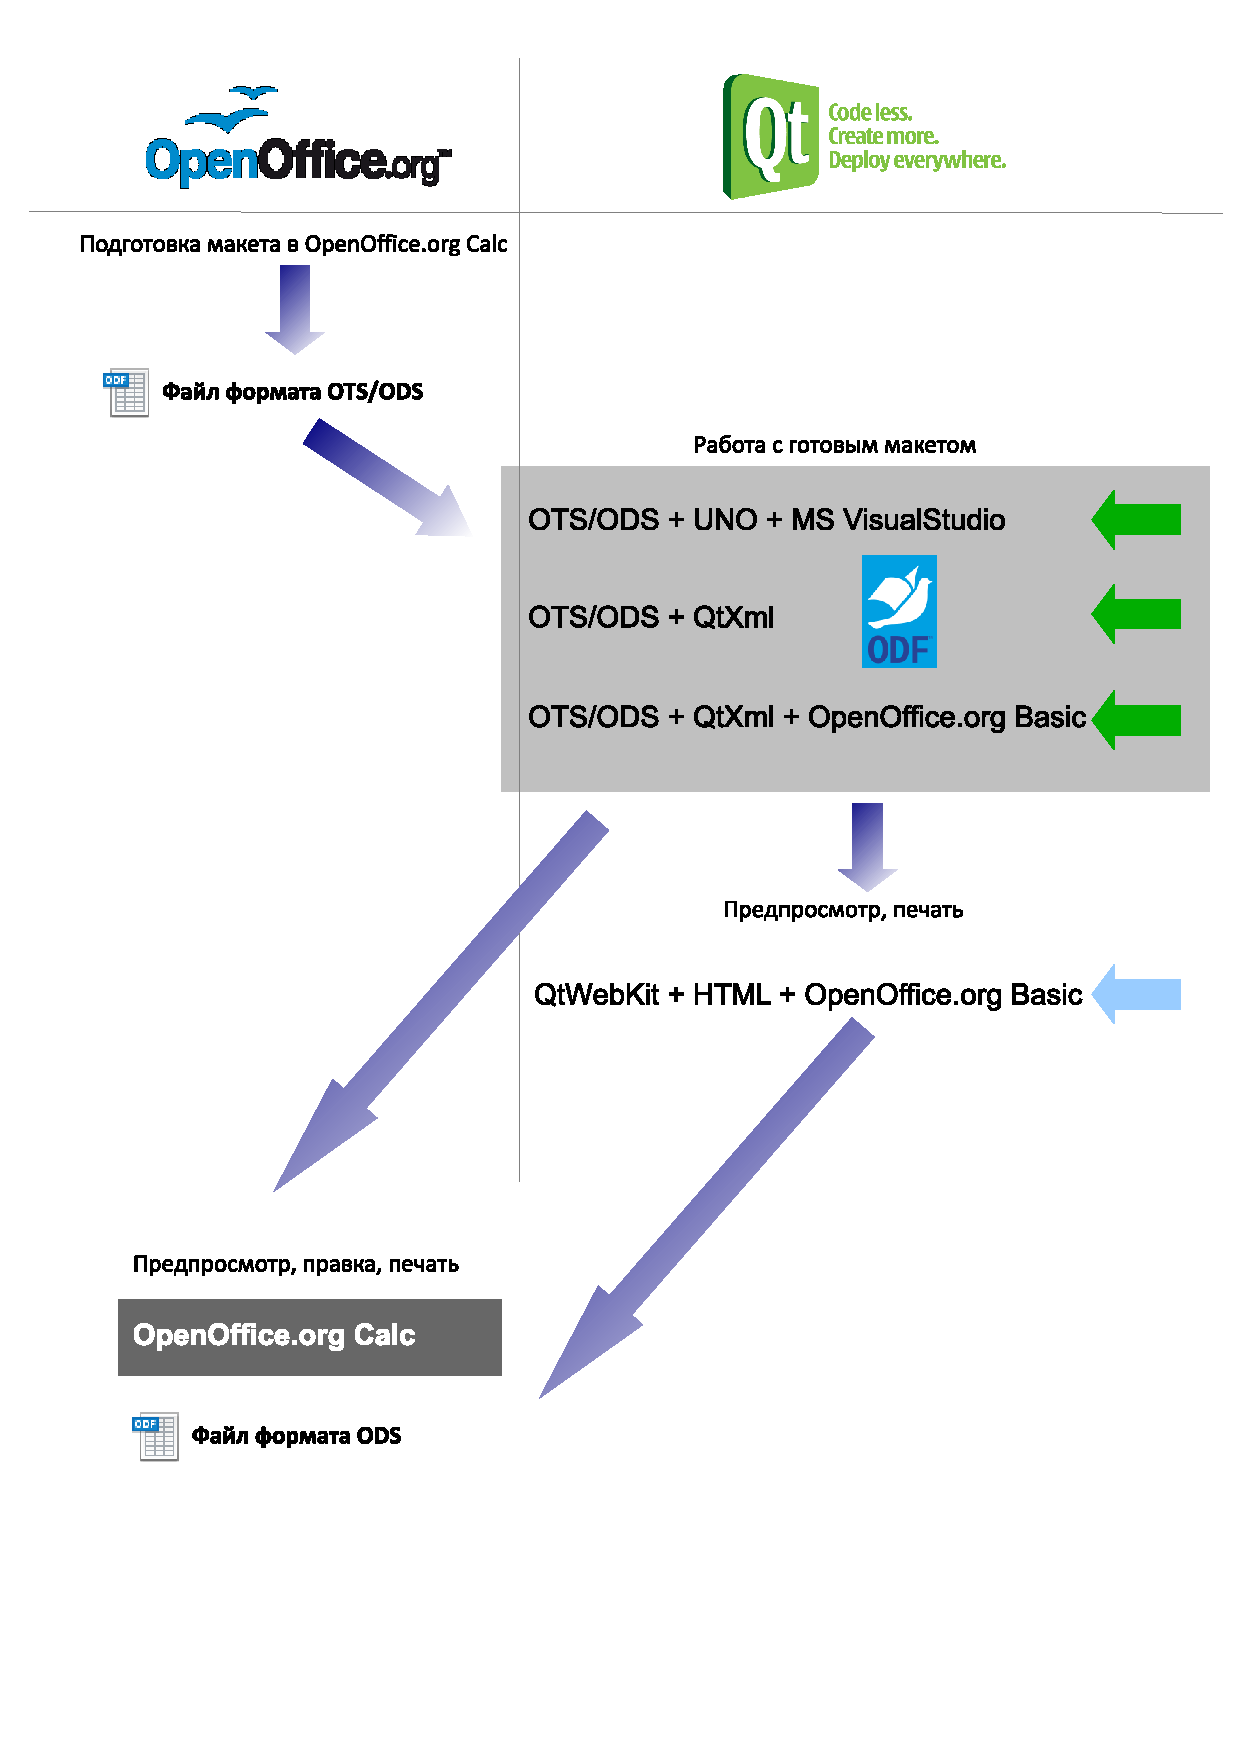
\includegraphics[width=8cm]{08_garanin}}
\end{figure}

\end{document}
